% Created by tikzDevice version 0.12.3 on 2021-05-23 17:18:31
% !TEX encoding = UTF-8 Unicode
\documentclass[10pt]{article}
\usepackage{tikz}
\usepackage{libertine}
\usepackage{amsmath}\begin{document}

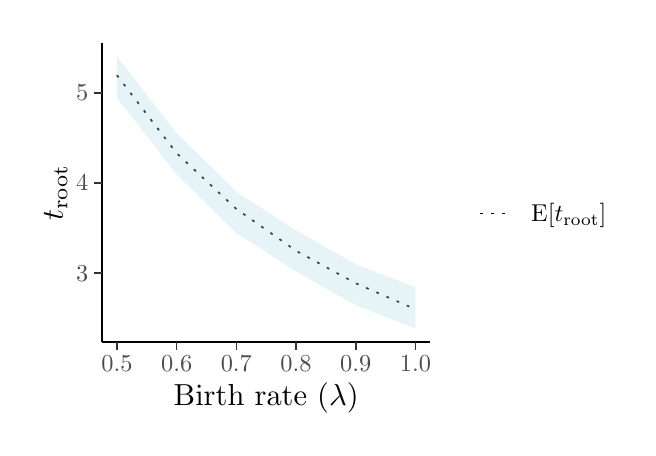
\begin{tikzpicture}[x=1pt,y=1pt]
\definecolor{fillColor}{RGB}{255,255,255}
\path[use as bounding box,fill=fillColor,fill opacity=0.00] (0,0) rectangle (216.81,144.54);
\begin{scope}
\path[clip] (  0.00,  0.00) rectangle (216.81,144.54);
\definecolor{drawColor}{RGB}{255,255,255}
\definecolor{fillColor}{RGB}{255,255,255}

\path[draw=drawColor,line width= 0.6pt,line join=round,line cap=round,fill=fillColor] (  0.00, -0.00) rectangle (216.81,144.54);
\end{scope}
\begin{scope}
\path[clip] ( 26.87, 30.91) rectangle (145.51,139.04);
\definecolor{fillColor}{RGB}{255,255,255}

\path[fill=fillColor] ( 26.87, 30.91) rectangle (145.51,139.04);
\definecolor{drawColor}{RGB}{0,0,0}

\path[draw=drawColor,line width= 0.6pt,dash pattern=on 1pt off 3pt ,line join=round] ( 32.26,127.35) --
	( 53.83, 99.16) --
	( 75.40, 79.03) --
	( 96.97, 63.93) --
	(118.54, 52.18) --
	(140.11, 42.79);
\definecolor{fillColor}{RGB}{173,216,230}

\path[fill=fillColor,fill opacity=0.30] ( 32.26,134.12) --
	( 53.83,106.40) --
	( 75.40, 85.19) --
	( 96.97, 71.31) --
	(118.54, 59.07) --
	(140.11, 50.68) --
	(140.11, 35.82) --
	(118.54, 44.22) --
	( 96.97, 56.46) --
	( 75.40, 70.34) --
	( 53.83, 91.55) --
	( 32.26,119.27) --
	cycle;
\end{scope}
\begin{scope}
\path[clip] (  0.00,  0.00) rectangle (216.81,144.54);
\definecolor{drawColor}{RGB}{0,0,0}

\path[draw=drawColor,line width= 0.6pt,line join=round] ( 26.87, 30.91) --
	( 26.87,139.04);
\end{scope}
\begin{scope}
\path[clip] (  0.00,  0.00) rectangle (216.81,144.54);
\definecolor{drawColor}{gray}{0.30}

\node[text=drawColor,anchor=base east,inner sep=0pt, outer sep=0pt, scale=  0.88] at ( 21.92, 53.00) {3};

\node[text=drawColor,anchor=base east,inner sep=0pt, outer sep=0pt, scale=  0.88] at ( 21.92, 85.55) {4};

\node[text=drawColor,anchor=base east,inner sep=0pt, outer sep=0pt, scale=  0.88] at ( 21.92,118.10) {5};
\end{scope}
\begin{scope}
\path[clip] (  0.00,  0.00) rectangle (216.81,144.54);
\definecolor{drawColor}{gray}{0.20}

\path[draw=drawColor,line width= 0.6pt,line join=round] ( 24.12, 55.88) --
	( 26.87, 55.88);

\path[draw=drawColor,line width= 0.6pt,line join=round] ( 24.12, 88.44) --
	( 26.87, 88.44);

\path[draw=drawColor,line width= 0.6pt,line join=round] ( 24.12,120.99) --
	( 26.87,120.99);
\end{scope}
\begin{scope}
\path[clip] (  0.00,  0.00) rectangle (216.81,144.54);
\definecolor{drawColor}{RGB}{0,0,0}

\path[draw=drawColor,line width= 0.6pt,line join=round] ( 26.87, 30.91) --
	(145.51, 30.91);
\end{scope}
\begin{scope}
\path[clip] (  0.00,  0.00) rectangle (216.81,144.54);
\definecolor{drawColor}{gray}{0.20}

\path[draw=drawColor,line width= 0.6pt,line join=round] ( 32.26, 28.16) --
	( 32.26, 30.91);

\path[draw=drawColor,line width= 0.6pt,line join=round] ( 53.83, 28.16) --
	( 53.83, 30.91);

\path[draw=drawColor,line width= 0.6pt,line join=round] ( 75.40, 28.16) --
	( 75.40, 30.91);

\path[draw=drawColor,line width= 0.6pt,line join=round] ( 96.97, 28.16) --
	( 96.97, 30.91);

\path[draw=drawColor,line width= 0.6pt,line join=round] (118.54, 28.16) --
	(118.54, 30.91);

\path[draw=drawColor,line width= 0.6pt,line join=round] (140.11, 28.16) --
	(140.11, 30.91);
\end{scope}
\begin{scope}
\path[clip] (  0.00,  0.00) rectangle (216.81,144.54);
\definecolor{drawColor}{gray}{0.30}

\node[text=drawColor,anchor=base,inner sep=0pt, outer sep=0pt, scale=  0.88] at ( 32.26, 20.19) {0.5};

\node[text=drawColor,anchor=base,inner sep=0pt, outer sep=0pt, scale=  0.88] at ( 53.83, 20.19) {0.6};

\node[text=drawColor,anchor=base,inner sep=0pt, outer sep=0pt, scale=  0.88] at ( 75.40, 20.19) {0.7};

\node[text=drawColor,anchor=base,inner sep=0pt, outer sep=0pt, scale=  0.88] at ( 96.97, 20.19) {0.8};

\node[text=drawColor,anchor=base,inner sep=0pt, outer sep=0pt, scale=  0.88] at (118.54, 20.19) {0.9};

\node[text=drawColor,anchor=base,inner sep=0pt, outer sep=0pt, scale=  0.88] at (140.11, 20.19) {1.0};
\end{scope}
\begin{scope}
\path[clip] (  0.00,  0.00) rectangle (216.81,144.54);
\definecolor{drawColor}{RGB}{0,0,0}

\node[text=drawColor,anchor=base,inner sep=0pt, outer sep=0pt, scale=  1.10] at ( 86.19,  7.86) {Birth rate ($\lambda$)};
\end{scope}
\begin{scope}
\path[clip] (  0.00,  0.00) rectangle (216.81,144.54);
\definecolor{drawColor}{RGB}{0,0,0}

\node[text=drawColor,rotate= 90.00,anchor=base,inner sep=0pt, outer sep=0pt, scale=  1.10] at ( 12.72, 84.97) {$t_{\text{root}}$};
\end{scope}
\begin{scope}
\path[clip] (  0.00,  0.00) rectangle (216.81,144.54);
\definecolor{fillColor}{RGB}{255,255,255}

\path[fill=fillColor] (156.51, 64.71) rectangle (211.31,105.24);
\end{scope}
\begin{scope}
\path[clip] (  0.00,  0.00) rectangle (216.81,144.54);
\definecolor{drawColor}{RGB}{0,0,0}

\path[draw=drawColor,line width= 0.6pt,dash pattern=on 1pt off 3pt ,line join=round] (163.45, 77.44) -- (175.02, 77.44);
\end{scope}
\begin{scope}
\path[clip] (  0.00,  0.00) rectangle (216.81,144.54);
\definecolor{drawColor}{RGB}{0,0,0}

\node[text=drawColor,anchor=base west,inner sep=0pt, outer sep=0pt, scale=  0.88] at (181.96, 74.55) {$\text{E}[t_{\text{root}}]$};
\end{scope}
\end{tikzpicture}

\end{document}
